\documentclass[12pt]{article}

\usepackage{times}
\usepackage{notes}
\usepackage{url}
\usepackage{graphicx}
\usepackage{amsfonts}

\begin{document}
\lecture{Artificial Intelligence}{HW02: Constraint Satisfaction}{CS 5300/6300, Spring 2012}
% IF YOU'RE USING THIS .TEX FILE AS A TEMPLATE, PLEASE REPLACE
% "CS5300/6300, Spring 2012" WITH YOUR NAME AND UID.

A paper copy of your answers are due at the beginning of class on the due date. We encourage using \LaTeX\ to produce your writeups. See the Homework Assignments page on the class website for details.

\section{Constraint Satisfaction}

Suppose a student, Tammy, wants to get a CS minor.  At Tammy's
university a CS minor consists of two required courses: (A)Computer
Science I, (B)Computer Science II; and three electives of which she
must take two (C)Discrete Math, (D)Algorithms, and (E)Computer
Architecture.

Like our own university, Tammy's has begun to enforce prerequisites.
Assume Computer Science I is a prerequisite for Computer Science II,
Computer Architecture, and Discrete Math; Discrete Math and Computer Science II are
prerequisites for Algorithms; and Computer Science II and Discrete Math
cannot be taken at the same time.

Luckily for Tammy each class is offered every semester, but she can
fit at most two CS courses on her schedule any given semester.  Tammy
wants to get her minor in 3 or fewer semesters.  We will model this
problem as a CSP where each class is a variable and the values
correspond to the remaining semesters till her graduation in Fall 2013
such that Fall 2012 = 1, Spring 2013 = 2, Fall 2013 = 3, and 0 means
Tammy does not take this course.

\begin{enumerate}

\item Find an assignment of variables to values by inspection which
  satisfies the constraints.

 \begin{solution}
$\{$ Computer Science I = 1, Computer Science II = 2, Computer Architecture = 2, Discrete Math = 3, Algorithms = 0 $\}$
 \end{solution}

\item Using the mathematical equality/inequality symbols ($=, <, >,
  \neq, \leq, \geq$), state the domain and constraints of the
  variables.

 \begin{solution}
$C = \{$ Computer Science I $<$ Computer Science II, Computer Science I $<$ Computer Architecture $OR$ Computer Architecture = 0, Computer Science I $<$ Discrete math $OR$ Discrete math = 0, Discrete Math $<$ Algorithms $OR$ Algorithms = 0, Computer Science II $<$ Algorithms $OR$ Algorithms = 0, Computer Science II $\neq$ Discrete Math, Computer Science I $\ge$ 1, Computer Science II $\ge$ 2, Computer Architecture + Computer Science II + Discrete Math + Algorithms $\ge$ 6, Computer Science II + Computer Architecture + Discrete Math + Algorithms $\le$ 8, Computer Science II + Discrete Math = 5 $\}$ \newline

Without considering the constraints, the domain for any particular $D_i = \{0, 1, 2\}$. The only node-consistent constraintes are for Computer Science I and Computer Science II; if we are allowed to consider these, then the domain for those two classes will shrink to $\{ 1,2,3\}$ and $\{2, 3\}$, respectively. If we want to do better, we will have to ensure arc-consistency (see the next section).
\end{solution}

\item Using back tracking search and arc consistency. Specifically run
  the AC3 algorithm described in the course notes and in the book as a
  preprocessor function and after each variable assignment.  If there
  is ambiguity in which variable to assign next you should select the
  one which comes first alphabetically.

  \begin{enumerate}

  \item What are the domain constraints after running AC3 on the initial CSP?

\begin{solution}
Given the constraints I have defined, our domains after the first preprocessing step would be $D_{CS I} = \{ 1, 2, 3 \}; D_{CS II} = \{ 2, 3 \}; D_{Architecture} = \{ 0, 1, 2, 3 \}; D_{Math} = \{0, 1, 2, 3 \}; D_{Algorithms} = \{ 0, 1, 2, 3 \}$.
\end{solution}
  
  \item What are the domain constraints after running AC3 on the
    assignment A = 1?

\begin{solution}
Given these constraints, an AC3 traversal will cause the domain to shrink a bit: $D_{CS I} = \{ 1 \}; D_{CS II} = \{ 2 \}; D_{Architecture} = \{ 0, 1, 2, 3 \}; D_{Math} = \{0, 1, 2, 3 \}; D_{Algorithms} = \{ 0 \}$.
\end{solution}
  
  \end{enumerate}

\item {\bf For graduate students only:} Assume Tammy wants to get her
  minor in just two semesters instead of three. Sketch a complete run
  of the AC3 algorithm with this new constraint and identify precisely
  when it will fail and how many states will be expanded before it
  fails.

% \begin{solution}
% \end{solution}

\end{enumerate}

\section{User Names}

Tammy has been accepted into the CS minor program and needs to choose
a user name for the computer lab. The computer lab at Tammy's
university enforces the following constraints on new user names:

\begin{enumerate}

\item User names may not be appending any string (including empty string) to the end of any existing user name.

\item User names may not be such that changing one letter of a name
  results in an existing user name.

\end{enumerate}

\noindent
For example if rat32 is a user name on the system Tammy would not be
able to select the rat321 (by constraint 1) or rot32 (by constraint 2).
How would you specify each constraint on new user name UN1 and existing user name UN2 using mathematical language?(use UN1[$i$] as the $i$th letter in UN1)

\begin{solution}
We solve this problem with a style of \textit{high-order constraints} described on page 206 of the book. \newline

Specifically, if UN2 is $n$ in length, then constraint 1 is really a matter of checking the first $n$ characters in both strings. Let us thus define an $n$-tuple of character equality comparisons: $\vec{Q} = \{equal(UN1[1], UN2[1]), \ldots, equal(UN1[n], UN2[n]) \}$, with the special case that, if UN1 is shorter than UN2, we return false for all the trailing characters. Further, let us define a function $count(\vec{T}) : \mathbb{R}^n \rightarrow \mathbb{Z}$ that takes some $n$-tuple of booleans, counts the number that are true, and returns this count. \newline

Then, constraint 1 simply translates to $n > 0, count(\vec{Q}) \neq n$; that is, $\vec{Q}$ compares the first $n$ characters in UN1 and UN2, so if we see that each of these is exactly the same, then clearly UN1 is simply UN2 concatenated with some other string, violating constraint 1. Further, the blank line is not a valid username, so $n > 0$. \newline

Constraint 2 requires slightly more work, since we must ensure both that UN1 and UN2 are the same length \textit{and} that there is not only one edit between them. Thus, let us define another vector of character comparisons, this time comparing the \textit{entirety} of both strings. Let us say that UN1 is $m$ characters in length, and that UN2 is $n$ characters in length. Further, let $t = \max(m,n)$. Then we can make a new $t$-tuple that comares all characters in both strings, $S = \{ equal(UN1[1], UN2[1]), \ldots, equal(UN1[t], UN2[t])$; note that (as above), if one of the strings ends before the others, the function $equal$ will simply return false for that character comparison. \newline

From here, constraint 2 is simple. First, since $t = \max(m,n)$, we know that $count(\vec{S}) = t$ indicates both that $m = n$ and that the usernames are equal. Further, if we know that $count(\vec{S}) = t-1$, then we know that the strings are equal \textit{except} for one character, which is either changed inside the string, or appended at the end of one of the strings. Since the first is disallowed by constraint 1, and the second is disallowed by constraint 2, our new constraint is: $count(\vec{S}) \neq t-1$
\end{solution}

\section{Map Coloring}

Consider the map:

% \centerline{\psfig{figure=hw2-1.eps,width=3in}}

% You don't have to print the figure. 
%\includegraphics[width=0.3\textwidth]{hw02-1.png}

\noindent
We want to find a coloring of this map such that no region touches a
region of the same color.

\begin{enumerate} 

\item First define what a variable is and then describe the domain,
  then using mathematical equality/inequality operators ($=, <, >,
  \neq, \leq, \geq$) describe the constraints assuming the number of
  colors you may use is 3.  A variable is a region of the map:
  1,2,3,4,5.  The domain would be a list of colors.

\begin{solution}
The set of variables will represent the color of a particular region, in this case given by $X = \{1,2,3,4,5,6\}$. The domain $D_i$ for any particular variable will be identical, and is merely a list of arbitrary colors: $D_i = \{ c1, \ldots, c_2 \}$. \newline

From here, the constraints will merely be a list of binary constraints that enforce no two contiguous regions are colored with the same color. We'll use the same abuse of notation on page 203, namely that we will denote a constraint simply as, for example, $region_i \neq region_t$, rather than the long hand $\{ (region_i, region_t), region_i \neq region_t \}$. Thus: $C = \{ 1 \neq 2, 1 \neq 3, 2 \neq 3, 2 \neq 5, 2 \neq 6, 3 \neq 4, 3 \neq 5, 4 \neq 5, 5 \neq 6 \}$
\end{solution}

\item Model this map as a graph of nodes and edges.  Explain why, in
  terms of nodes and edges, it is impossible to have a two color
  solution to this problem.

\begin{solution}
A graphical representation of this map is included below. There is a very good reason why we can't have only a two-color solution to this graph, and we don't even need to look at the whole graph to know why. If you just look at nodes $1$, $2$, and $3$, then you can see that they are all connected to each other. There is no way to use two colors such that the constraints are fulfilled. \newline

Specifically, pick any of those 3 nodes and give it one color. This means that the other two nodes connected to it must be the other of the two colors. But, no matter which node you picked, the other two are always connected to each other, so the must also be different. But because we only have two colors, they can't be without violating the constraint and being the same color as the original node. Contradiciton. Since these 3 nodes can't possibly be colored subject to these constraints, and since adding more nodes around them can't fix this problem, this graph cannot be colored using only two colors. \newline

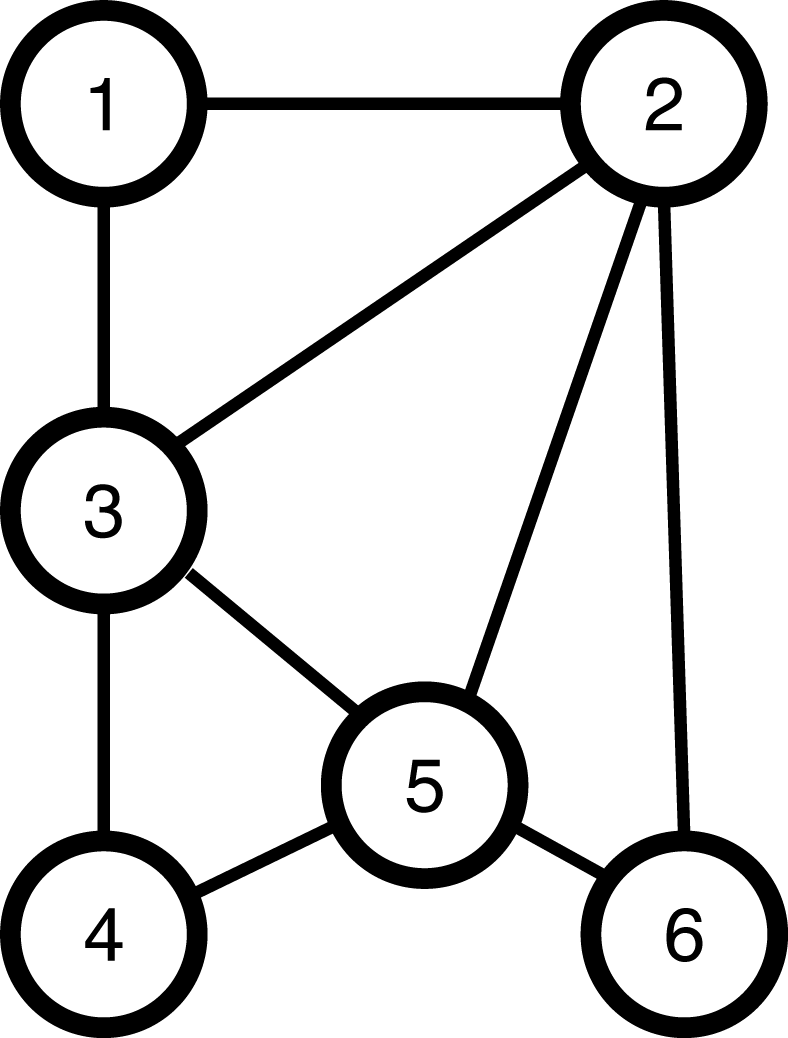
\includegraphics[scale=0.5]{mapgraph.png}
\end{solution}

\item {\bf For graduate students only:} suppose the map changes:

%\centerline{\psfig{figure=hw2-2.eps,width=3in}}

% You don't have to print the figure. 
% \includegraphics[height=0.3\textwidth]{hw02-2.png}
 
  \begin{enumerate}

  \item Draw a graph representing this map.

% \begin{solution}
% \end{solution}

  \item What is the new minimum number of colors that can be used to
   color this map such that no regions of the same color are touching?

% \begin{solution}
% \end{solution}

  \end{enumerate}

\end{enumerate}

\end{document}
